\section{Results and discussion}


\subsection*{Metrics}
\label{sec:metrics}
Two metrics were used to assess the performances of the models. 
The first metric is the Weighted Interval Score (WIS), which is a metric commonly used in forecast evaluation (see \cite{cramer2022evaluation} or \cite{paireau2022ensemble}). 

Let $\alpha$ be in $]0, 1[$. Let $\hat{y}$ be the prediction of the model and $y$ the real value.
Let $[l, u]$ be the $(1-\alpha)$ confidence interval of the prediction.
We define the Interval Score ($IS$) as: \\
$IS_\alpha([l, u], \hat{y}, y) = \frac{2}{\alpha} \times (\mathbb{1}_{\{y<l\}} (l-y) + \mathbb{1}_{\{y>u\}} (y-u) + (u-l))$. \\
This metric is made of three terms: a term of overprediction that punishes a model predicting a confidence interval which is above the real value, a term of underprediction that punishes a model whose confidence interval is under the real value, and a term of range, that punishes too wide confidence intervals. \\
Let $(\alpha_k)_{k \in \{1, \dots , K\}} \in ] 0 , 1 [ ^K $
The WIS is defined as follow. \\

$WIS([l, u], \hat{y}, y) = \sum_{k=0}^{K} w_k IS_{\alpha_k}([l, u], \hat{y}, y) $ , with $(w_k)_{k \in \{1, ... , K\}} \in \mathbb{R}_+ ^K $ weights chosen by the user. \\

According to previous literature (\cite{cramer2022evaluation}), I decided to set \\
$(\alpha_k)_{k \in \{1, ... , K\}} = [0.02, 0.05, 0.1, 0.2, 0.3, 0.4, 0.5, 0.6, 0.7, 0.8, 0.9]$ and $ \forall k \in  \{1, ... , K\}, w_k = \frac{\alpha_k}{2}$
One can notice that the WIS does not take into account the point prediction, but focuses on confidence interval accuracy. \\

The second metric chosen is the Root Mean Square Error ($RMSE$). 
With the same notations as above, we define the $RMSE$ as follow: \\
$RMSE([l, u], \hat{y}, y) = \sqrt{(y-\hat{y})^2}$\\
This metric focuses on the point prediction, and does not take into account the confidence intervals. 


The models were tested on all the 324 pandemics, on 14 data points different (at days 20, 40, 60, ..., 280). 
For each individual point, the models were trained on the previous days of the pandemic. 
A 7 and 14 days ahead prediction was asked, and $[0.02, 0.05, 0.1, 0.2, 0.3, 0.4, 0.5, 0.6, 0.7, 0.8, 0.9]$ confidence-intervals were computed. 
The WIS and the RMSE of these predictions were then computed. 
For the analysis of the results, I decided to remove the points for which the number of hospitalized was below 100, as both point classification and model predictions were irrelevant at this period of the pandemic.
Moreover, it is senseless to assess the performances of the models during the period in which there is no pandemic, as the interesting models are the ones that can predict the number of hospitalized during the waves.
Not removing those points would lead to biased results, as they represent 44\% of the dataset, and we would have concluded that the best model is the one that performs well when there is no pandemic. 
\subsection{Point classification}
\label{sec:classification}

In order to compare the performance of the models at different point of the pandemic, I have  classified the points in six categories: \textit{stable, increase, big increase, decrease, big decrease}.
The $R_{eff}$ number was used for the point classification. 
This number is easily available from the Covasim simulation. 
$R_{eff}$ represents the expected number of people that an infected person will infect.
For a pandemic $X_{i, i \in [1, ..., n]}$ of reproduction number $R_{i, i \in [1, ..., n]}$, and a day $d \in [1, \hdots, n]$, the classification is made according the following rule: \\
\begin{itemize}
    \item if $X[d]$<100: \\
    classification = "no pandemic"
    \item Elif $R[d] <0.5$: \\
    classification = "big decrease"
    \item Elif $R[d] < 0.8$: \\
    classification = "decrease"
    \item Elif $R[d] < 1.2$: \\
    classification = "stable" 
    \item Elif $R[d] < 3$: \\
    classification = "increase"
    \item Else: \\
    classification = "big increase"
\end{itemize}


The values of the thresholds were chosen by hand. 
As the model are tested on the days [20, 40, 60, ..., 280], we labelled all of these points with the function described above. 
It resulted that among all those 4536 points, 698 were classified as 'big decrease', 579 as 'decrease', 388 as 'stable', 752 as 'increase',  132 as 'big increase', and 1987 as 'no pandemic'.



\subsection{Evaluation of the models}

The models described above were tested on 14 points of each of the 324 pandemics generated, when the pandemic was significant (i.e when more than 0.01\% of the population was hospitalized, in our case when the value of the number of hospitalized was above 100). 
For each point, two  predictions were made:  a 7-days ahead and a 14-days ahead. 
Each prediction was evaluated thanks to WIS and RMSE (see \ref{sec:metrics}), and then ranked according to the performances of other models.
The points of evaluation were also classified in one of the following categories: 'big increase', 'increase', 'stable', 'decrease' and 'big decrease', based on the value of the reproductive number at this time of the pandemic (see:\ref{sec:classification} for more details). 
It is then possible to get global information on the rankings of the models. 
For instance, if the loss and the reach of prediction is fixed, we can look at the distribution of rankings of all the models for a type of point (to see the best model for a type of point), as in Fig.\ref{fig:rankings}.
\begin{figure}[h!]
    \centering
    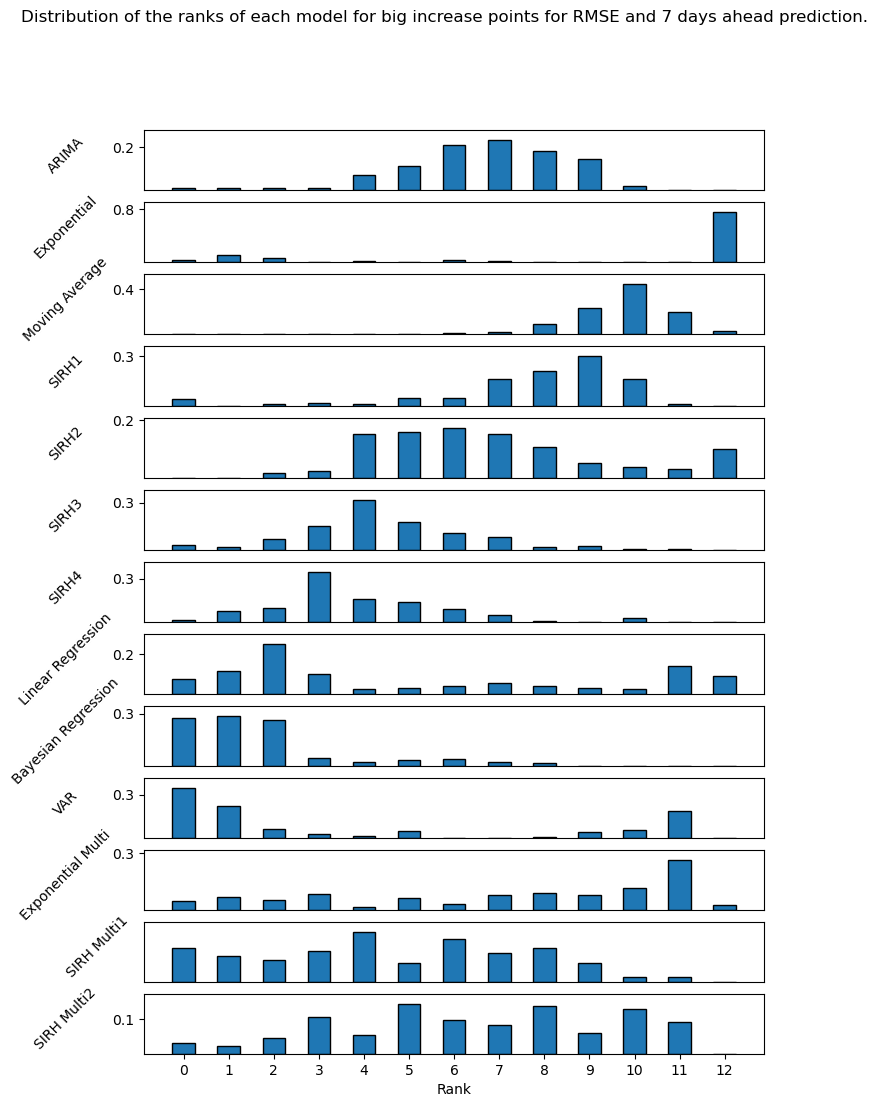
\includegraphics[width=0.5\textwidth]{figures/ranks_big_increase_RMSE_7.png}
    \caption{Distribution of rankings of the models for big increase points for 7-days ahead predictions and RMSE loss}
    \label{fig:rankings}
\end{figure}
This distribution of rankings of the model can be summed up in one single value: the expected value of the rank of a model (see Fig.\ref{fig:expected_rank}), which enables to get the idea of the best model for this type of point, this loss, and this prediction range on a more compact figure. 

\begin{figure}[h!]
    \centering
    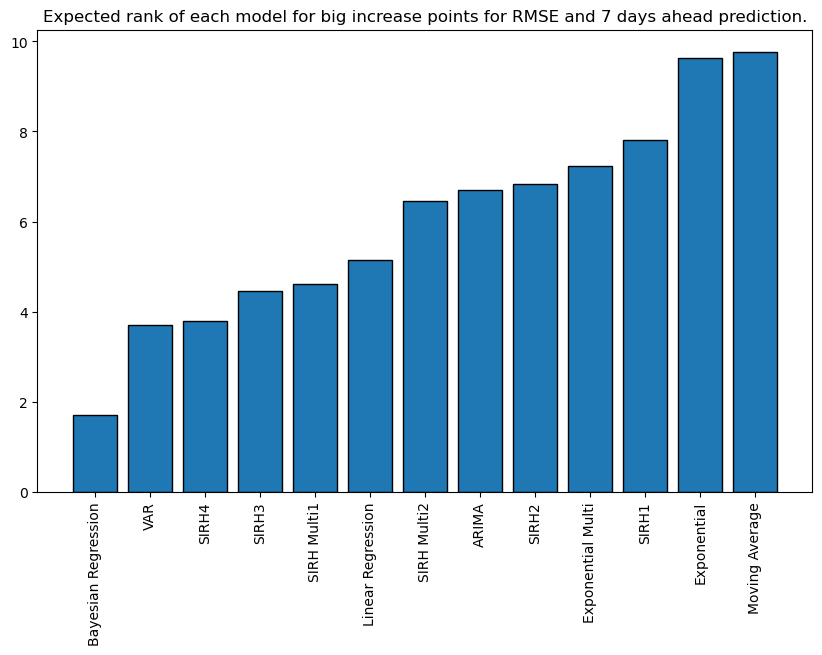
\includegraphics[width=0.5\textwidth]{figures/expected_ranks_big_increase_RMSE_7.png}
    \caption{Expected rank of the models for big increase points for 7-days ahead predictions and RMSE loss}
    \label{fig:expected_rank}
\end{figure}

This new number loses information (for instance on bimodal rankings distribution) but enables to highlihgt the expected performance of a model. 
For each loss and range of prediction, the expected rank of the models for each type of point can be vizualized on the same figure, which enables to have a global look of the performances of the models.(Fig.\ref{fig:heatmap_RMSE_7}) 
\begin{figure}[h!]
    \centering
    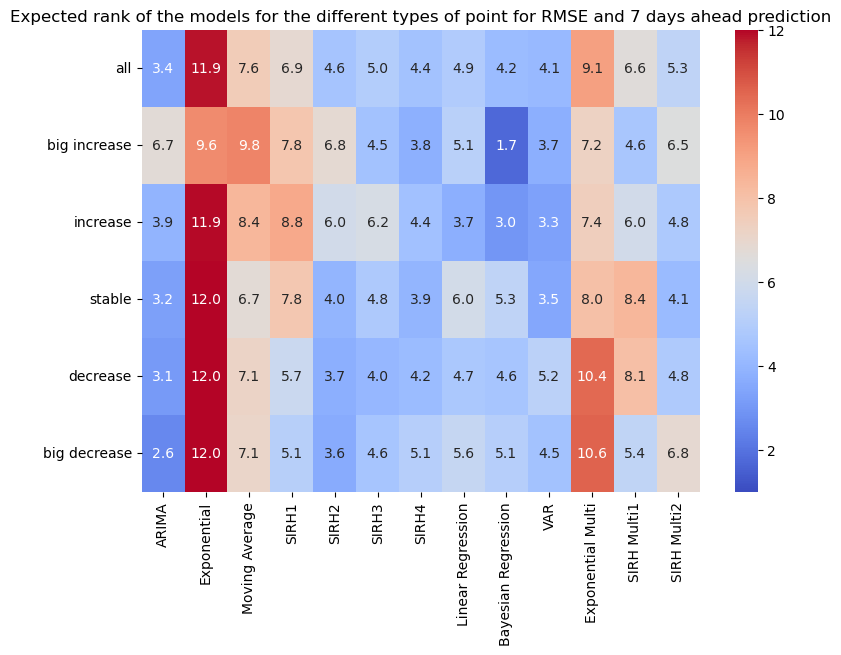
\includegraphics[width=0.7\textwidth]{figures/heatmap_RMSE_7.png}
    \caption{Expected rank of the models for each type of point for 7-days ahead predictions and RMSE loss. For instance, the Bayesian Regression has an average ranking of 1.7 on all the 'big increase' points of the 324 pandemics generated }
    \label{fig:heatmap_RMSE_7}
\end{figure}


The other heatmaps corresponding to RMSE for 14 days ahead prediction and WIS for 7 and 14 days ahead predictions can be found in the appendix (\ref{sec:appendix}).
Some general interpretations can be made on these results. 
I noticed that regressors performances drop from 7-days ahead to 14-days ahead. 
The family of the SIRH model does slightly better for long terms predictions than for short term ones. 
The ARIMA performance drops from 7-days ahead to 14-days ahead predictions. 
The exponential models are very bad and almost always the last ones. 

\subsection{The Ensemble model}
The performance of the ensemble models have to be separated from the performances of the other models. 
Indeed, as the ensemble models were trained on a part of the pandemics, they can't be evaluated on the whole set of outbreaks. 
The performances discussed in this part refer to the same evaluation as above, but only for the RMSE loss and on a test set that represents 20\% of the pandemics. 
The performances of these two models are shown in the two figure below (Fig.\ref{fig:esb_rank_7} and Fig.\ref{fig:esb_rank_14})

\begin{figure}[htbp]
    \centering
    \begin{subfigure}[b]{0.45\textwidth}
        \centering
        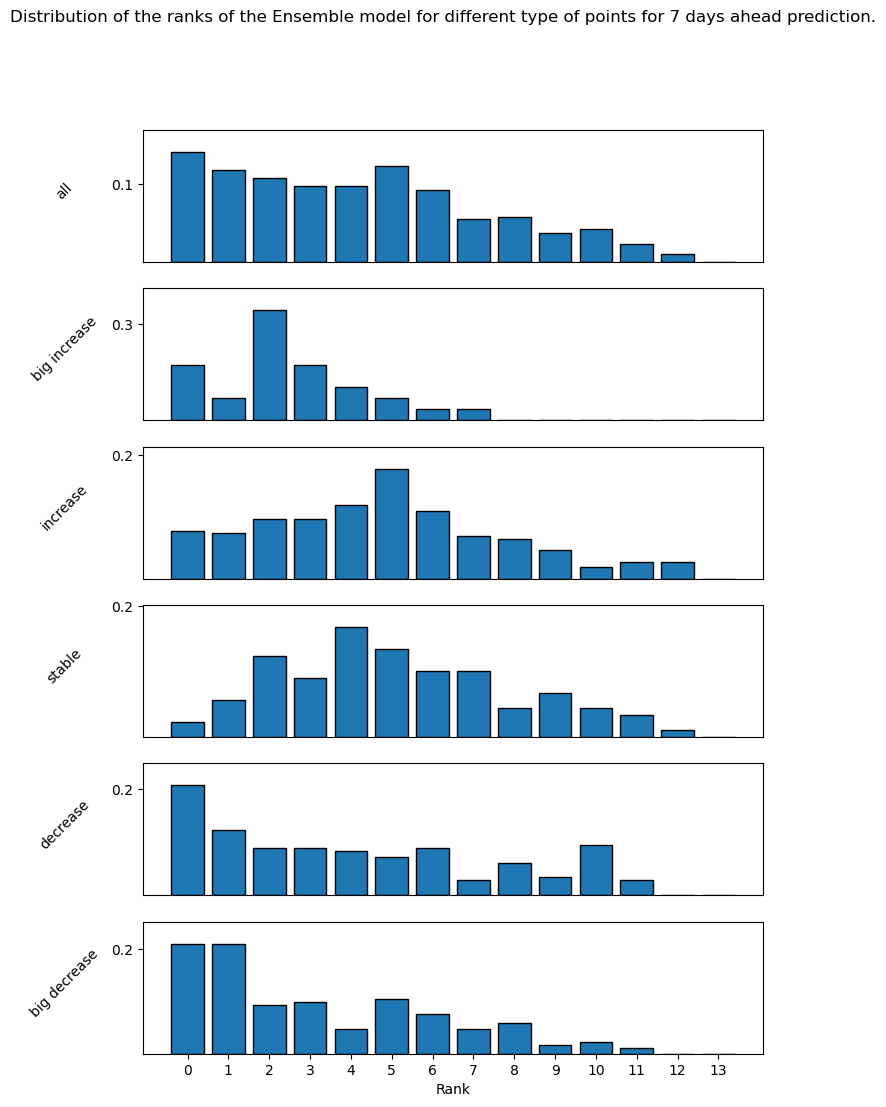
\includegraphics[width=\textwidth]{figures/esb_rank_7.png}
        \caption{Expected rank of the ensemble model for each type of point for 7-days ahead predictions and RMSE loss}
        \label{fig:esb_rank_7}
    \end{subfigure}
    \hfill
    \begin{subfigure}[b]{0.45\textwidth}
        \centering
        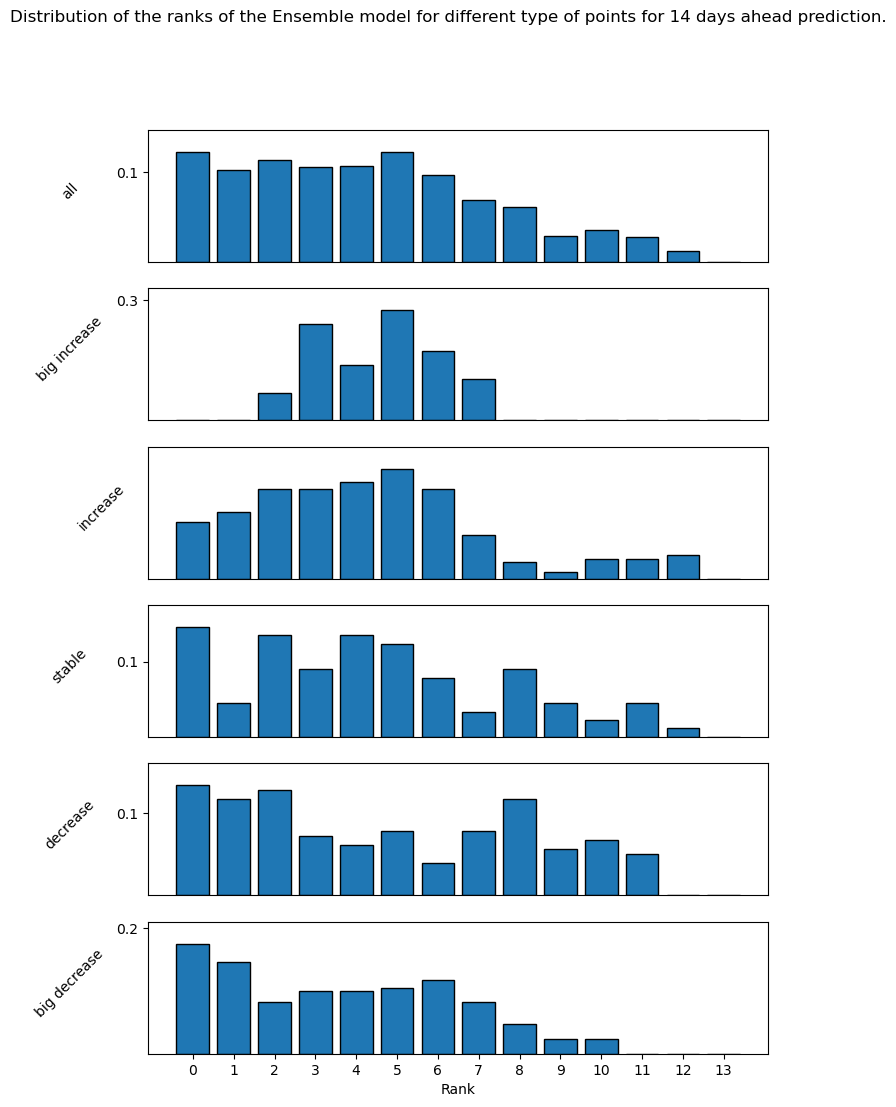
\includegraphics[width=\textwidth]{figures/esb_rank_14.png}
        \caption{Expected rank of the ensemble model for each type of point for 14-days ahead predictions and RMSE loss}
        \label{fig:esb_rank_14}
    \end{subfigure}
    \caption{Comparison of expected ranks for 7-days and 14-days ahead predictions}
    \label{fig:esb_rank_comparison}
\end{figure}

The distribution of the ranks of the ensemble model is almost always on the left side of the x-axis.
It is a very consistent model, and almost always in the top models. 
The heatmaps of expected ranks on all type of points enables to see how consistent is the ensemble model (Fig.\ref{fig:heatmap_esb_7} and Fig.\ref{fig:heatmap_esb_14}) compared to the other models. 


\begin{figure}[htbp]
    \centering{
    \begin{subfigure}[b]{0.45\textwidth}
        \centering
        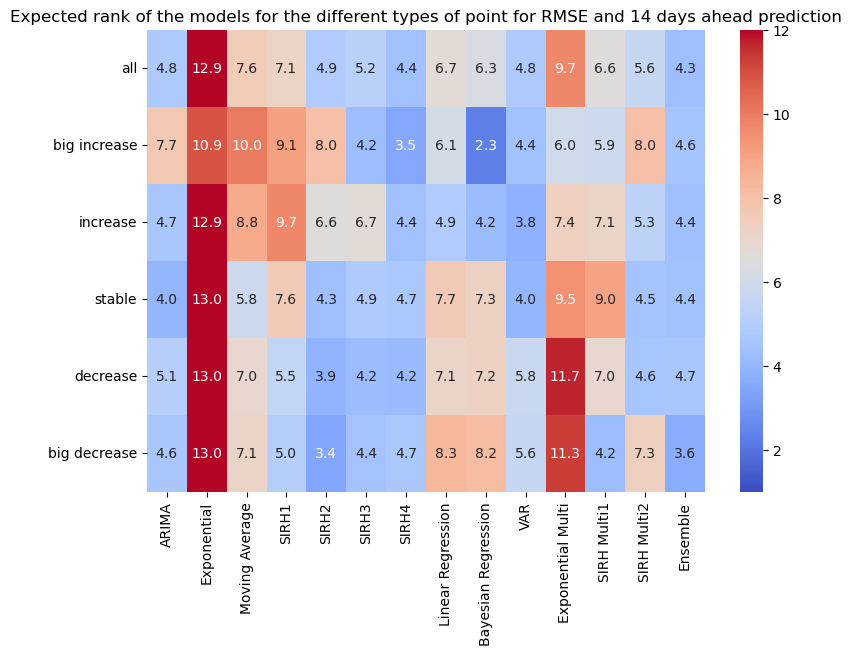
\includegraphics[width=\textwidth]{figures/heatmap_esb_14.png}
        \caption{Expected rank of all the models for each type of point for 14-days ahead predictions}                                              
        \label{fig:heatmap_esb_14}
    \end{subfigure}
    \begin{subfigure}[b]{0.45\textwidth}
        \centering
        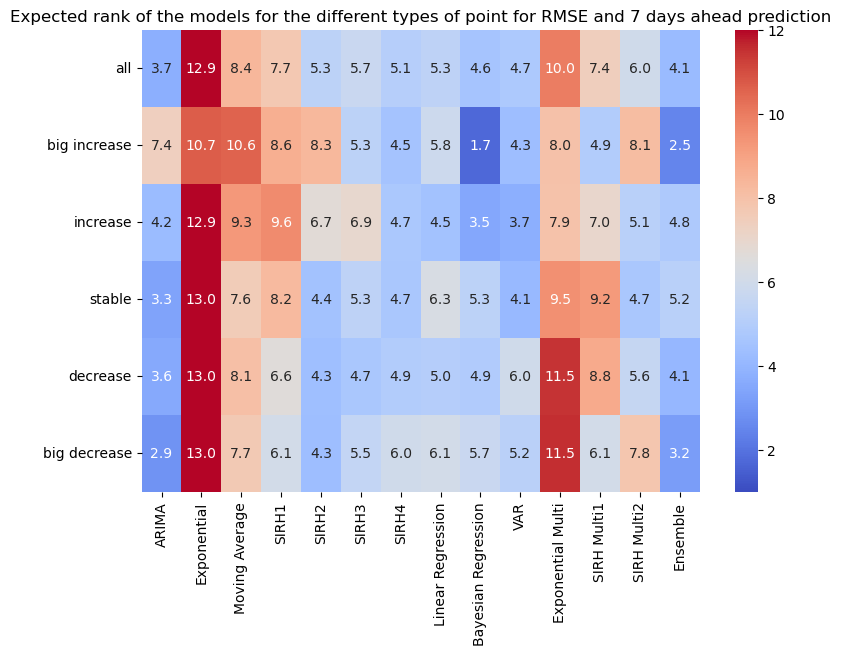
\includegraphics[width=\textwidth]{figures/heatmap_esb_7.png}
        \caption{Expected rank of all the models for each type of point for 7-days ahead predictions}
        \label{fig:heatmap_esb_7}
    \end{subfigure}}
    \caption{Expected rank of all the models for each type of point and RMSE loss on the test set for 7-days and 14-days ahead predictions}
    \label{fig:heatmap_esb_comparison}
\end{figure}

From these figures, one can notice that the ensemble model is rarely the best, but never the last model. 
Indeed, for a loss, a type of point and a prediction range, one can look at the best models in terms of expected rank.
For instance, on the Fig.\ref{fig:expected_rank}, one can see that the top 3 models are Bayesian Regression, VAR and SIRH4. 
On the train set, the Ensemble model is the only model that appears in all top-6 models for all types of points, all losses and all prediction ranges.
Its consistency allows for accurate predictions and helps avoiding outlier predicted values that sometimes appear on the other good models (such as VAR and ARIMA). 



\subsection{Summary of Key Findings}

This method enabled us to assess the consistency of the different models that were implemented. 
Indeed, comparing the models on a set of diverse pandemics enlighted the most consistent with the different pandemics.
Moreover, the classification of the models with the type of points leads to the determination of the phase of the pandemic in which each model is the best, and on the other hand to assess which model is the best for a given $R_{eff}$ . 
This result is promising, as the reproduction number is a quantity often estimated by the stakeholders during a pandemic. 
The interpretation based on the heatmaps Fig.\ref{fig:heatmap_RMSE_14}, Fig.\ref{fig:heatmap_RMSE_7} and Fig.\ref{fig:heatmap_WIS_14} and Fig.\ref{fig:heatmap_WIS_7} show the following results: \\



\begin{itemize}
    \item Arima and VAR are very effective models in terms of expected ranking. They are the two best models for 7-days ahead predictions and in the top 4 models for the 14-days ahead predictions. 
    \item Adding information with the mobility and the number of infected is not beneficial for the models. We observe almost always a poorer performance of the models of the second type compared to their equivalent model of the first type (VAR / Arima and SIRH Multi / SIRH). Only the exponential multi outperforms the mere exponential model, but as they both perform pretty bad, this result is not interesting. 
    \item The autoregressive models (Bayesian and Linear Regression, ARIMA and VAR) perform best for short term predictions rather than long term ones. On the other hand, the SIRH models, which have a physical meaning and try to fit the data to an understandable model perform better for long term predictions. This is also observed in the coefficients of the ensemble model (see Fig. \ref{fig:ensemble_weights}). Indeed, the ensemble model puts more weight on the VAR and Arima models for short term predictions and more on the SIRH models for long terms predictions.  
    \item The difference of ranking between the models is more pronounced when we rank them with RMSE rather than WIS. This might be due to the fact that the confidence intervals are not well calibrated and that the real value always land outside it. 
    \item The Moving Average model is not the worst model and is often ranked between 6 and 8. This might be due to the fact that as the curve of the number of hospitalized is continuous, the mean never diverge too much from the real value, while other models might misinterpret the trend of the curve and land far away from the real value. 
    \item The Exponential models are almost always the last models, except for big increase points that are almost always at the very beginning of the pandemic. the fact that the beginning of a pandemic looks like an exponential curve is also shown with the SIRH model, when the number of infected is very small. 
    \item The Ensemble model performs quite well. I noticed that it is very rarely the best model for a type of point, while other models almost always have some points on which they make the best prediction. On the other hand, it is never the last, and has a very consistent ranking: it is the only model that appears in all top-6 models for all types of points, all losses and all prediction ranges.
\end{itemize}



\subsection{Test on real data}


I also tested the models on real data from the Covid-19 pandemic in Sweden and in France. 
The data of the number of hospitalized individuals was taken from the website \href{https://ourworldindata.org/covid-hospitalizations}{Our World in data}, the data of the number of infected was taken from the website \href{ https://www.worldometers.info/coronavirus/country/sweden/#coronavirus-cases-linear}{Worldometers}, and the mobility used was the mobility from the \href{https://www.google.com/covid19/mobility/}{ Google reports}, see \cite{google_covid19_mobility}. 
As the mobility used in the previous part concerned public transportation mobility, I decided to focus on the relative mobility in the public transports (\textit{transit\_stations\_percent\_change\_from\_baseline} in the .csv file provided by Google).
The models were tested each 20 days from the 2nd of March to the 7th of December 2020. 
For each of these points, the models were trained on the data from the beginning of the pandemic to the day before the prediction, and outputed a 7-days ahead and a 14-days ahead prediction. 
As I wanted to compare the models with the ensemble model, I decided to assess their performances with the RMSE and not the WIS. 
For each point prediction, the models were ranked according to the RMSE between the prediction and the real value. 
The rankings are shown on Fig.\ref{fig:rankings_real_data}. 
The predictions of the models are plotted with the real data on Fig.\ref{fig:real_data}, in the appendix. 
I noticed similar results to what I observed on the synthetized set for Arima, VAR, Bayesian and Linear regressors: they perform well, but have better results for short term predictions rather than long ones. 
The performance of the ensemble model is disappointing during the period between the 20th of July and the 8th of October for the Swedish data, but not for the French one, which is surprising, as the curve are both shaped with two waves. 
Moreover, the Ensemble model puts lots of weight on the VAR model (see fig \ref{fig:ensemble_weights}), which might be very sensitive to the errors in the data, as it takes into account the number of infected and the mobility.
The difference between this two countries might therefore be due to the quality of the estimation of the number of infected. 
However, during this "flat" period,  even if the ensemble model is not well-ranked, it lands not far from the real value, the other models being better because they are a little closer than him (only for 7 days ahead predictions). 
On French data, the ensemble model performs well, and is very consistent. 
The difference of performance between the two countries might also be te consequence of the difference of range of the pandemics due to the difference of population between the two countries. 

 



\subsection{Comparison with Previous Research}

The very good performance of both VAR and ARIMA models is consistent with previous research. 
\cite{kufel2020arima} and \cite{shang2021regional} both assess the performance of the ARIMA model in terms of regional or national prediction accuracy. 
The interpretation of the coefficients of the ARIMA model enables to have information on the inherent parameters of the pandemic, or to discover links between the different regions of a country. 
The consistency of the ensemble model has been shown in many previous studies (see \cite{cramer2022evaluation}, \cite{VIBOUD201813} and \cite{reich2019accuracy}), who also observe that their ensemble model outperformed any individual model. 
They also observe the fact that the ensemble model is very consistent: rarely the best, but never the last, allowing to produce robust forecasts. 
In \cite{rahmandad2022enhancing}, the authors compared several model to understand they key features that enabled a model to make long term predictions. 
These features are: " \textit{(1) capturing the physics of transmission (instead of using black-box models); (2) projecting human behavioral reactions to an evolving pandemic; and (3) resetting state variables to account for randomness not captured in the model before starting projection.}"
These findings are consistent with the results that I have observed. 
Indeed, I have showed that the SEIR model (capturing the physics of transmission and resetting state) performances increase from 7-days ahead to 14-days ahead predictions, while black-box models (such as Arima or VAR), are less effective for long terms prediction. 
This has to be qualified, as the "long term predictions" of this report refer to a 14-days ahead prediction, while the study \cite{rahmandad2022enhancing} get interested to predictions up to 14-weeks reach. 

The methodology of point classification has not be found in any other paper of the literature. 
Some studies assess the performance of the models during different times of a pandemic (see \cite{howerton2023evaluation}), but this systematic point classification based on the reproduction number was not found. 

\subsection{Practical Implications}

This study might be useful when facing a new pandemic.
As the value of the $R_{eff}$ is often estimated by the researchers during a pandemic, it could be used to decide which type of model to use during the current pandemic. 


\subsection{Limitations}

During my researchs, I didn't take into account the impact of uncertainity of the data on the models. 
Indeed, the Covasim library provided a daily data of high quality and without any noise, but
real-life data is often full of mistakes, of missing values or of time-lag in the reports (\cite{greene_Nowcasting}).
It would be interesting to measure the robustness of the models with respect to these imperfections to assess if the models can still make good predictions, and to focus on the robustness of the ensemble model. 
Moreover, the models of the second type used the number of infected to predict the number of hospitalized. 
This quantity is not directy accessible and is often estimated with tests, which could lead to huge variations in the predicted values.  
Finally, the models were only tested on outbreaks generated with Covasim, which might introduce bias in the results, despite the effort to create a diverse set of pandemics. 
